Table~\ref{tab:main-results} reports operational error and coverage; Figure~\ref{fig:contrasts} presents every primary comparison.
\begin{table*}[t]
\centering\small
\caption{Operational user-macro MAE and valid-output coverage. Invalid reader arrays use the predeclared constant-3 fallback. Numerical methods always produce valid predictions. Native memory is evaluated on Coat only. Lower MAE is better.}
\label{tab:main-results}
\begin{tabular}{lrrrr}
\toprule
System / evidence & Coat MAE & Valid & MovieLens MAE & Valid\\
\midrule
History mean & 0.991 & 200/200 & 0.839 & 200/200\\
History median & 0.923 & 200/200 & 0.817 & 200/200\\
History-only ridge & 0.914 & 200/200 & 0.845 & 200/200\\
Qwen / no history & 1.694 & 199/200 & 1.029 & 197/200\\
Qwen / full history & 1.074 & 200/200 & 0.937 & 195/200\\
Qwen / permuted history & 1.218 & 200/200 & 0.957 & 196/200\\
Qwen / native memory & 1.158 & 198/200 & -- & --\\
Phi / no history & 1.236 & 177/200 & 0.986 & 141/200\\
Phi / full history & 0.910 & 185/200 & 0.921 & 199/200\\
Phi / permuted history & 1.115 & 180/200 & 0.950 & 199/200\\
Phi / native memory & 1.059 & 184/200 & -- & --\\
\bottomrule
\end{tabular}
\end{table*}

\begin{figure*}[t]
\centering
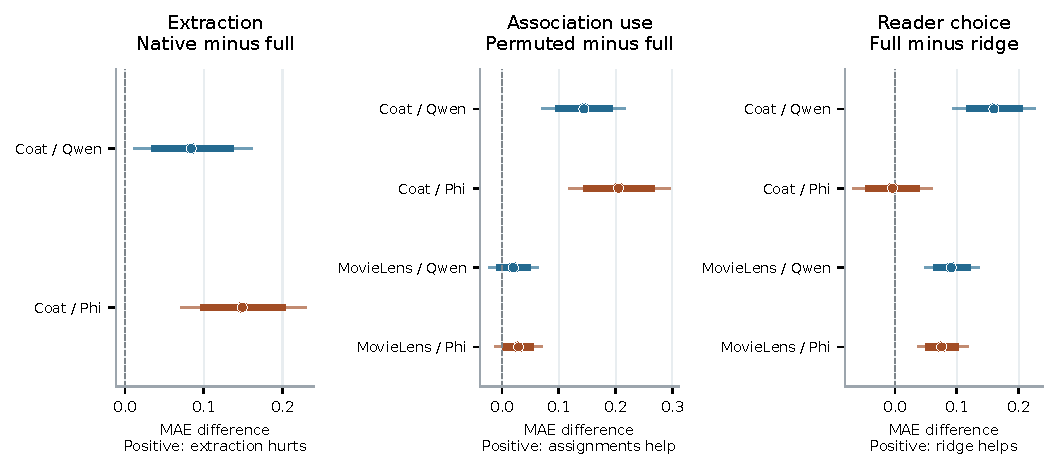
\includegraphics[width=\textwidth]{../results/figures/confirmation/primary-contrasts.pdf}
\caption{All ten predeclared contrasts in user-macro MAE. Points show paired means; thick bars are ordinary 95\% percentile intervals and thin bars are family-adjusted 99.5\% intervals. Positive values mean extraction increases error, correct assignments help, or ridge has lower error, respectively. Each all-user comparison contains 200 users.}
\label{fig:contrasts}
\end{figure*}

\subsection{The tested native pipeline increases Coat error}
On Coat, Qwen's MAE rises from 1.074 with full history to 1.158 with native memory, a paired increase of $0.084$ (family-adjusted interval $[0.012,0.160]$). Phi's MAE rises from 0.910 to 1.059, an increase of $0.149$ ($[0.072,0.229]$). Both intervals exclude zero. Relative to the full-history point estimates, these increases are 7.8\% and 16.4\%, respectively. These relative percentages are descriptive, not separately bootstrapped effects.

Both native-memory conditions nevertheless have lower MAE than their no-history counterparts (Table~\ref{tab:main-results}). Thus a favorable memory-versus-no-history comparison would miss a measurable loss relative to the supplied source. This result concerns the complete tested construction-and-reading pipeline. It does not identify whether omissions, inferences, formatting, or reader responses to the representation account for the loss.

The paired common-valid extraction differences remain positive: $0.084$ across 198 Qwen users and $0.147$ across 171 Phi users. Their adjusted intervals also exclude zero. This sensitivity supports the direction of the operational result without relying solely on fallback predictions, although validity-based selection can change the evaluated population.

\subsection{Association use depends on the domain}
Permuting historical assignments increases Coat MAE by $0.144$ for Qwen ($[0.072,0.215]$) and $0.205$ for Phi ($[0.119,0.295]$). The rating multiset is identical on both sides of each comparison. The audit also confirms identical full/permuted prompt-token counts for every user and reader. Consequently, neither rating-level information nor input length explains these differences. Correct assignments provide useful evidence under both readers in this task.

MovieLens yields smaller effects: $0.020$ for Qwen ($[-0.022,0.062]$) and $0.029$ for Phi ($[-0.011,0.069]$). Both adjusted intervals include zero. Phi's ordinary all-user 95\% interval narrowly excludes zero, but its common-valid 95\% interval does not. We therefore do not describe MovieLens as a confirmed positive replication of the association effect. The same evaluation procedure applies in both domains, but the positive Coat finding does not automatically generalize.

The already-frozen numerical control shows the same domain pattern: permuting history raises ridge MAE by 0.215 on Coat and 0.019 on MovieLens. These descriptive differences are outside the ten primary tests. They suggest weaker usable association signal under this MovieLens representation and sample, rather than uniquely implicating the language-model readers.

Secondary ordering diagnostics provide additional context. On Coat, full-history pairwise concordance is 0.550 for Qwen and 0.599 for Phi, versus 0.487 and 0.496 under permutation. On MovieLens the corresponding values are 0.520 and 0.551, versus 0.493 and 0.508. These are descriptive summaries, not additional multiplicity-adjusted tests, and can reflect shared item effects as well as individual preferences.

\subsection{Reader choice and metric choice change the conclusion}
The history-only ridge reader achieves MAE 0.914 on Coat and 0.845 on MovieLens. Its advantage over Qwen full history is $0.160$ on Coat ($[0.095,0.225]$) and $0.091$ on MovieLens ($[0.049,0.135]$). It also improves on Phi in MovieLens by $0.076$ ($[0.038,0.117]$). The Coat Phi-minus-ridge difference is $-0.004$ ($[-0.067,0.059]$), which does not establish either system's superiority or equivalence. These comparisons match supplied history and metadata, not pretraining or computation.

Ridge is not uniformly best by every metric. MovieLens history median has a lower descriptive MAE, 0.817, despite assigning every target the same prediction and therefore attaining concordance 0.5. Ridge has concordance 0.558 and a lower RMSE, 1.042 versus 1.127. On Coat, Phi's full-history MAE is close to ridge, but its RMSE is higher (1.249 versus 1.136) and concordance lower (0.599 versus 0.637). These differences show why a scalar rating-error ranking cannot stand in for all aspects of personal prediction.

\subsection{Reliability and cost are part of the measurement}
Across 2,800 reader calls, 150 outputs fail the fixed contract. Qwen has 3 invalid calls on Coat and 12 on MovieLens; Phi has 74 and 61. Failures are condition-dependent: 59 of Phi's MovieLens no-history calls are invalid, compared with one in each history condition. The constant-3 reference has MAE 1.236 on Coat and 0.984 on MovieLens, providing context for no-history performance. Gains over no history should therefore not be interpreted as pure representational gains: the operational contrast also includes reader priors and output reliability. There are no reader transport errors. Of the 150 invalid outputs, 35 terminate at the token limit and 115 violate the output contract after normal termination. All remain in the operational analysis; no answer is retried or repaired.

The 200 native writes produce 2,830 stored entries, including one empty store after a length-limited response. Writing consumes 1,974,104 model tokens. Reading native memory uses 20.7\% fewer prompt tokens than full history for Qwen and 22.3\% fewer for Phi on Coat, but this excludes the initial writing cost. Smaller read inputs accompany greater prediction error in this experiment, so compression alone is not evidence of a favorable deployment tradeoff.

The separate checker reconstructs all 2,800 reader inputs and verifies 4,600 user-system records and all ten primary contrasts. The maximum continuous-metric discrepancy is below $2.1\times10^{-14}$. A further source-data-free verifier regenerates aggregate statistics and bootstrap intervals from the 5,400 released per-user error summaries, including supplementary baselines. These checks validate computational consistency, not external peer review. Complete metrics, paired sensitivities, failure categories, and resource totals appear in Appendix~\ref{app:metrics}.
